\subsection{合成工作负载下的性能评估}
\label{subsec:sgxdedup-synthetic}

本文使用一组随机文件组成一个合成工作负载数据集,其中每个文件均仅包含全数据集范围内非重复的数据块(完全随机)。 默认情况下,本文将随机文件大小设置为2\,GiB(Exp\#2除外,本文在其中对消息锁加密密钥生成性能进行了压力测试)。 客户端通过云服务端上传或下载文件。为了避免磁盘I/O对性能的影响,本文将随机文件存储在内存中而不是磁盘上(Exp\#8除外,本文在真实云环境部署中使用磁盘处理随机文件数据集)。本文的结果为10次运行的平均结果以及T分布(\textit{Student's t-Distribution})下的95\%置信区间包含在条形图中(为简洁起见,本文在折线图中不标注置信区间)。

\paragraph*{Exp\#1(单客户端消息锁加密密钥生成)。}本文评估\sysnameS 中两轮消息锁加密密钥生成的效率。首先,客户端基于Rabin指纹(\S\ref{sec:sgxdedup-implementation})对2\,GiB随机文件进行可变长度分块,并产生数据块指纹,发出消息锁加密密钥生成请求。然后,客户端为另一个2\,GiB随机执行相同步骤进行密钥生成。不同之处在于第二轮密钥生成将使用预先计算的加解密掩码加速密钥安全区处理(\S\ref{subsec:sgxdedup-encryption})。

本文将\sysnameS 的单客户端消息锁加密密钥生成速度与现有服务器辅助密钥生成方案进行了对比。本文考虑两种基于OPRF协议的密钥生成方法,即\textit{OPRF-BLS}\cite{armknecht2015transparent}和\textit{OPRF-RSA}\cite{bellare2013DupLESS},它们分别基于盲BLS签名和盲RSA签名实现了OPRF原语(\S\ref{subsec:sgxdedup-problem})。此外,本文还考虑了两种较宽松的密钥生成方法,即\textit{MinHash encryption}\cite{qin17}和\textit{TED}\cite{li2020TED},它们以存储效率和安全性为代价换取密钥生成性能。具体来说,MinHash encryption使用OPRF-RSA协议基于每个数据段(较数据块更大的单位,平均大小为1\,MiB)中所有数据块指纹的最小值产生消息锁加密密钥。TED使用数据块的短哈希、密钥服务器的全局秘密以及基于草图(Sketch)统计的数据块频率共同为每个数据块生成消息锁加密密钥(参见\cite{li2020TED}中的\S3.3)。

\begin{figure}[!htb]
    \centering
    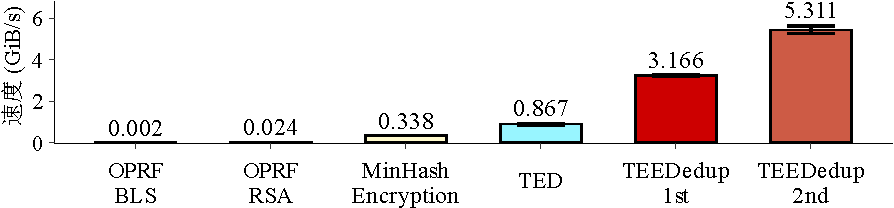
\includegraphics[width=0.8\textwidth]{pic/sgxdedup/plot/exp_a2/expa2_keyGenPerformance.pdf}
    \caption{(Exp\#1)单客户端消息锁加密性能对比}
    \label{fig:sgxdedup-keygen-comparison}
\end{figure}

图~\ref{fig:sgxdedup-keygen-comparison}显示了测试结果。\sysnameS 通过避免OPRF-BLS、OPRF-RSA和MinHash encryption中昂贵的密码原语以及TED中的频率计数等计算,实现了远超所有对比对象的密钥生成性能。\sysnameS 的第一轮密钥生成相比OPRF-BLS和OPRF-RSA实现了1,583倍和131.9倍的性能提升。与MinHash encryption和TED(两者均牺牲了部分存储效率和安全性)相比,分别提高了9.4倍和3.7倍。而第二轮基于推测性加密,\sysnameS 将第一轮的消息锁加密密钥生成速度再次提高了67.8\%。

\paragraph*{Exp\#2(多客户端消息锁加密密钥生成)。}为了对密钥生成安全区的密钥生成性能进行压力测试,本文采用一台设备通过多线程模拟福哦个客户端,同时向密钥服务器(在不同的设备上运行)发出消息锁加密密钥生成请求。这里,每个模拟客户端仅包含一个线程用于发出密钥生成请求(随机生成数据块指纹)。

由于密钥安全区中可存储的加解密掩码至多可用于处理约11.25\,GiB的原始数据(\S\ref{subsec:sgxdedup-encryption}),为了在第二轮密钥生成中为每个模拟的客户端均启用推测性加密,本文将将每个模拟客户端配置为生成40,960个指纹(约满足320\,MiB原始数据的密钥生成需求),并将密钥安全区离线计算加解密掩码的客户端数量配置为与模拟客户端数量一致。使得第二轮密钥生成中,所有客户端的所有密钥生成请求均通过推测性加密进行处理。本文统计分析所有模拟客户端聚合的密钥生成速度,该速度定义为总密钥生成数量除以第一个客户端启动到所有客户端全部完成密钥生成的时间。

\begin{figure}[!htb]
    \small
    \centering
    \begin{tabular}{@{}c@{}c@{}c}
        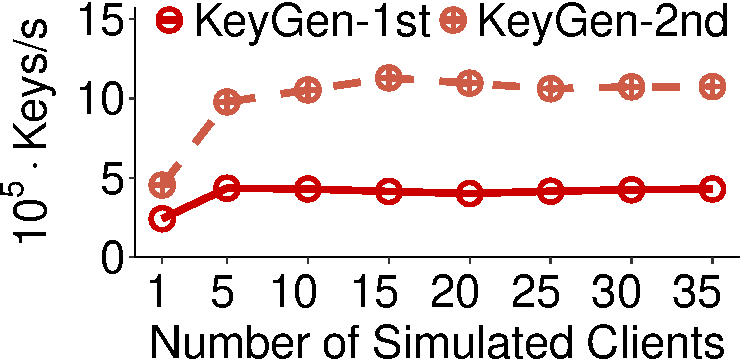
\includegraphics[width=0.49\textwidth]{pic/sgxdedup/plot/exp_a3/expa3_keyScale_performance_number_singleThread.pdf} & 
        \hspace{5pt}
        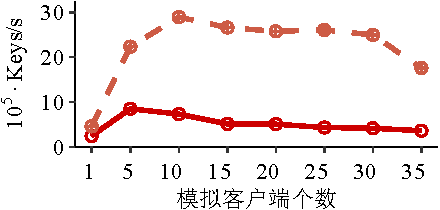
\includegraphics[width=0.49\textwidth]{pic/sgxdedup/plot/exp_a3/expa3_keyScale_performance_number_multiThread.pdf}     \\
        \mbox{\small (a)密钥安全区单线程执行}                                                                               & 
        \mbox{\small (b)密钥安全区多线程执行}                                                                                  \\
    \end{tabular}
    \caption{(Exp\#2) 多客户端消息锁加密密钥生成}
    \label{fig:sgxdedup-exp-keygen-scalability}
\end{figure}

图~\ref{fig:sgxdedup-exp-keygen-scalability}(a)显示了密钥安全区仅使用单个线程处理所有模拟客户端的密钥生成请求时的聚合密钥生成速度。在第一轮和第二轮密钥生成中,\sysnameS 分别在5个和15个客户端时达到最大生成速度($4.3\times 10^5$\,keys/s和$11.3\times 10^5$\,keys/s)。随后,受限于单核处理能力上限,密钥生成速度基本保持不变。图~\ref{fig:sgxdedup-exp-keygen-scalability}(b)显示了密钥安全区多线程服务模拟客户端时的密钥生成聚合速度。第一轮和第二轮密钥生成分别在5个和10个模拟客户端时实现了最高$8.5\times 10^5$\,keys/s和$29\times 10^5$\,keys/s的密钥生成速度,随后由于CPU上下文切换开销逐渐增大,聚合速度逐渐下降。平均而言,第二轮基于推测性加密相较于第一轮实现了4.4倍的聚合密钥生成加速。

\paragraph*{Exp\#3(密钥生成批量大小的影响)。}

本文首先使用Exp\#1的方法来评估请求密钥生成的指纹批量大小对密钥生成速度的影响。图~\ref{fig:sgxdedup-exp-keygen-breakdown}(a) 显示了两轮密钥生成速度与请求的指纹批量大小的关系。当指纹批量大小从$1$更改为$2^{15}$时,第一轮和第二轮的密钥生成速度分别从0.0086\,GiB/s增加到3.3\,GiB/s以及从0.0091\,GiB/s增加到6.5\,GiB/s。图~\ref{fig:sgxdedup-exp-keygen-breakdown}(b)去除网络传输开销后分别统计了客户端及密钥安全区在生成1\,MiB原始数据的消息锁加密密钥时分别的计算开销。密钥安全区和客户端的时间消耗随着指纹批量的增大而减少,这是因为更大的批量大小意味着要为所有指纹批次计算的MAC更少(参见\S\ref{sec:sgxdedup-implementation})。此外,密钥安全区的时间开销随着批量大小增加在第一轮中从2.0\,ms减少到0.2\,ms,在第二轮从 1.8\,ms减少到0.1\,ms。时间开销明显减少的原因是较大的指纹批量大小避免了过多次调用密钥生成安全区内调用(key generation Ecall),并减少了CPU的上下文切换开销。

\begin{figure}[!htb]
    \centering
    \begin{tabular}{@{\ }c@{\ }c}
        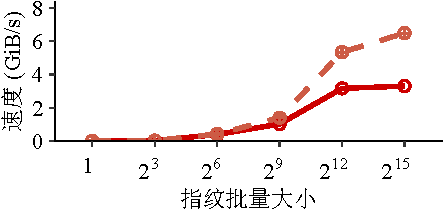
\includegraphics[width=0.48\textwidth]{pic/sgxdedup/plot/exp_a2/expa2_keyEnclaveBatchSize_Performance_overall.pdf} & 
        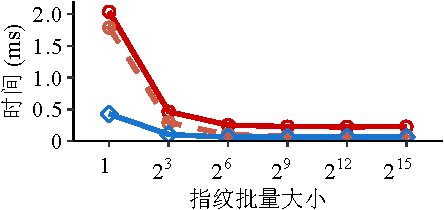
\includegraphics[width=0.48\textwidth]{pic/sgxdedup/plot/exp_a2/expa2_keyEnclaveBatchSize_Performance_1st.pdf}        \\
        \mbox{\parbox{0.48\textwidth}{\small (a) 总体密钥生成速度vs.批量大小}}                                             & 
        \mbox{\parbox{0.48\textwidth}{\small (b) 密钥生成中的计算开销vs.批量大小}}
    \end{tabular}
    \caption{(Exp\#3)指纹批量大小对密钥生成性能的影响}
    \label{fig:sgxdedup-exp-keygen-breakdown}
\end{figure}


\paragraph*{Exp\#4(自会话密钥的更新延迟)。}在自更新会话密钥管理中,密钥安全区和云服务端通过密钥回归独立地执行密钥更新,其方法是从旧密钥状态导出新密钥状态(\S\ref{subsec:sgxdedup-key-management})。本文评估密钥安全区和云服务端中的密钥更新延迟。

\begin{figure}[!htb]
    \centering
    \begin{tabular}{@{\ }c@{\ }c}
        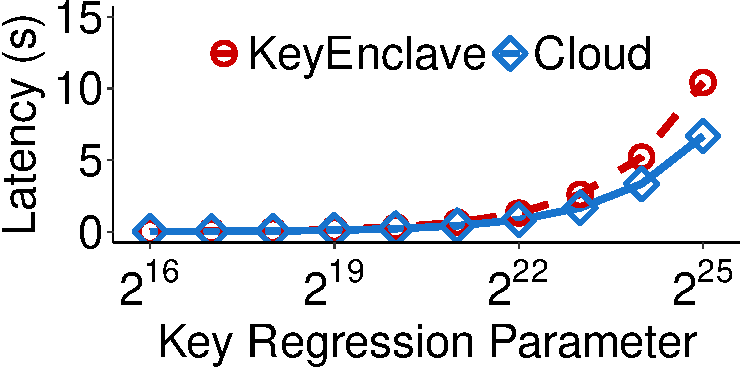
\includegraphics[width=0.48\textwidth]{pic/sgxdedup/plot/exp_a5/expa5_keyRegression_time.pdf} & 
        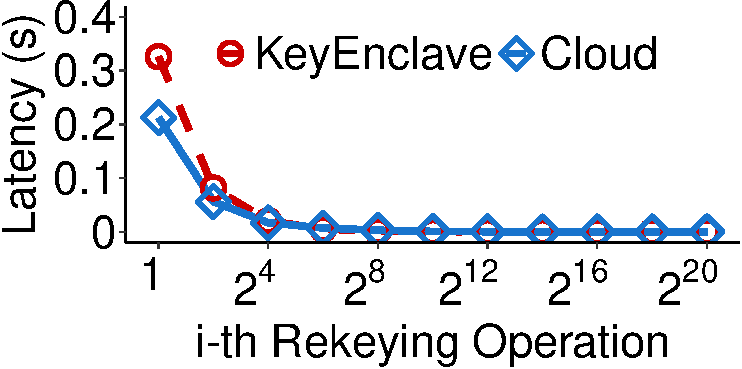
\includegraphics[width=0.48\textwidth]{pic/sgxdedup/plot/exp_a5/expa5_keyRegression_time_default.pdf} \\
        \mbox{\small (a)不同密钥回归参数}                                                             & 
        \mbox{\small (b)不同密钥回归次数}
    \end{tabular}
    \caption{(Exp\#4)会话密钥更新延迟}
    \label{fig:sgxdedup-rekeyingLatency}
\end{figure}

图~\ref{fig:sgxdedup-rekeyingLatency}(a)显示了会话密钥的首次更新延迟与密钥回归参数(即,可承受的最大密钥更新次数,参见\S\ref{subsec:sgxdedup-key-management})的关系。密钥安全区和云服务端的密钥首次密钥更新延迟随着密钥回归参数的增大而增加,因为更大的密钥回归参数意味着密钥更新中的哈希计算更多。由于安全区处理密集计算的能力较弱\cite{harnik2018SGX},这里密钥安全区的密钥更新延迟相较云服务端高1.22-1.56倍。

图~\ref{fig:sgxdedup-rekeyingLatency}(b)显示了每次会话密钥更新操作的延迟,此时初始化的密钥回归参数固定为2$^{20}$。随着执行更多的密钥更新操作,密钥更新延迟逐渐减少,每次密钥更新操作均可相较于上一次密钥更新操作节省一次哈希计算。平均而言,密钥安全区的密钥更新延迟为0.040\,s。相比之下,云服务端约为0.027\,s,这意味着密钥更新开销是有限的。

\paragraph*{Exp\#5 (数据所有权证明计算开销)。}本文评估\sysnameS 的数据所有权证明性能。本文考虑一个对2\,GiB随机文件执行数据所有权证明的客户端。客户端从该文件中创建明文数据块,加密每个明文数据块,并向云服务端发出数据所有权证明请求。本文根据客户端(所有权证明安全区对密文数据块计算指纹并产生相应签名)和云服务端(验证指纹对应的数据的真实性)中所有数据块的总计算时间来测量所有权证明计算开销。本实验中的速度计算排除了客户端和云服务端之间的网络传输时间开销(本文在Exp\#10中考虑了网络传输时间)。

本文将\sysnameS 与两种最先进的数据所有权证明方法进行比较:(i)\textit{PoW-MT}\cite{halevi11}(halevi等人提出的基本版本),该数据所有权证明方法使用纠删码对块进行编码,并在编码的内容上构建Merkle树用于所有权证明;(ii)\textit{PoW-UH}\cite{xu2013weak}建立在通用哈希之上,相较于PoW-MT牺牲部分安全性以换取更高的性能。为了公平比较,本文使用C++复现了PoW-MT和PoW-UH方法。此外,halevi等人\cite{halevi11}提出了改进的数据所有权证明方法,但它们均为了更低的内存开销产生了更大的性能开销。

\begin{figure}[!htb]
    \begin{minipage}[t]{0.47\textwidth}
        \centering
        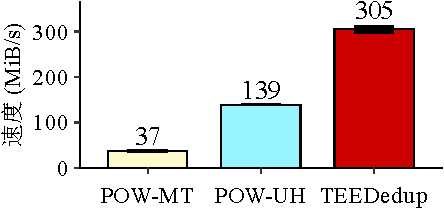
\includegraphics[width=\linewidth]{pic/sgxdedup/plot/exp_a4/expa4_powPerformance.pdf}
        \caption{\small(Exp\#5)数据所有权证明的\\计算性能(不含网络开销)}
        \label{fig:sgxdedup-pow-comparison}
    \end{minipage}%
    \hspace{0.2in}
    \begin{minipage}[t]{0.47\textwidth}
        \centering
        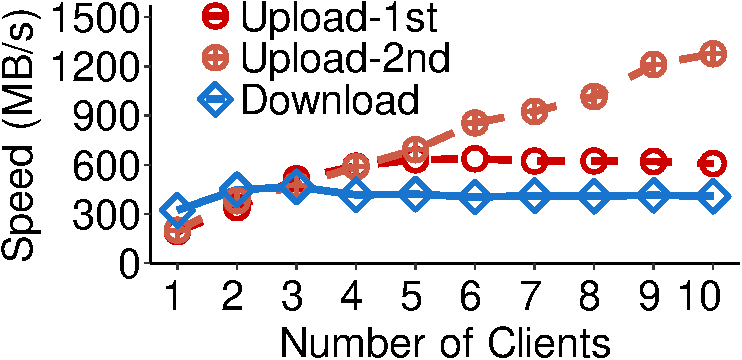
\includegraphics[width=\linewidth]{pic/sgxdedup/plot/exp_b1/expb1_multiple_client.pdf}
        \caption{(Exp\#9)多客户端聚合的\\上传/下载性能}
        \label{fig:sgxdedup-multiClientThroughput}
    \end{minipage}%
\end{figure}

图~\ref{fig:sgxdedup-pow-comparison}显示了性能测试结果。由于\sysnameS 避免了客户端中的纠删码编码和Merkle树构造,其实现了相较于PoW-MT高达8.2倍的性能提升。此外,\sysnameS 相较于安全性较弱的PoW-UH实现了2.2倍的性能提升。

\paragraph*{Exp\#6(密文数据块批量大小对基于TEE的所有权证明的性能影响)。}本文评估密文数据块批量大小对\sysnameS 的数据所有权证明性能的影响。与Exp\#5中仅考虑数据所有权的整体计算速度相反,本实验评估数据所有权证明的有效性能。有效性能的定义为输入的2\,GiB随机文件的大小与从密文数据块输入安全区开始到全部完成指纹和证明生成、云端验证(包含网络传输开销)的总时间的比率。本文禁用了客户端上传数据块和云服务端执行重复数据删除的操作,以减少性能测量噪声。

\begin{figure}[!htb]
    \centering
    \begin{tabular}{@{\ }c@{\ }c}
        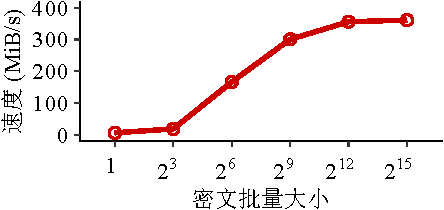
\includegraphics[width=0.48\textwidth]{pic/sgxdedup/plot/exp_a4/expa4_powBatchSize_overall.pdf} & 
        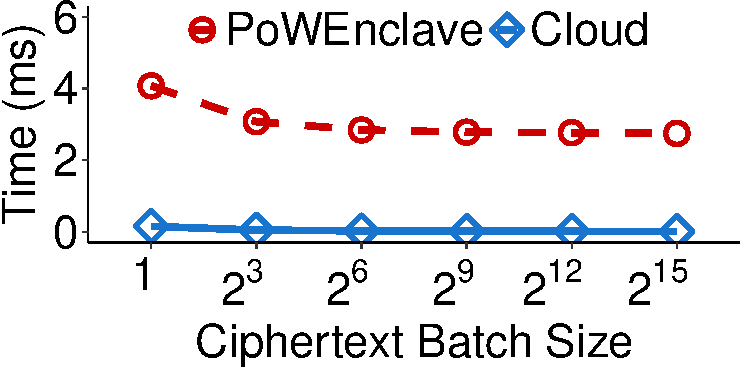
\includegraphics[width=0.48\textwidth]{pic/sgxdedup/plot/exp_a4/expa4_powBatchSize_breakdown.pdf}  \\
        \mbox{\parbox{0.48\textwidth}{\small (a) 所有权证明有效速度vs.批量大小}}                        & 
        \mbox{\parbox{0.48\textwidth}{\small (b) 所有权证明的计算开销vs.批量大小}}
    \end{tabular}
    \caption{(Exp\#6)密文数据块批量大小对所有权证明的性能影响}
    \label{fig:sgxdedup-exp-pow-impact}
\end{figure}

图~\ref{fig:sgxdedup-exp-pow-impact}(a)显示了数据所有权证明有效性能与不同密文数据块批量大小的关系,可以发现随着密文数据块批量大小增加,数据所有权证明性能从6.2\,MiB/s提升到360.9\,MiB/s。图~\ref{fig:sgxdedup-exp-pow-impact}(b)显示了所有权证明安全区和云服务端在数据所有权证明中每处理1\,MiB数据时所需的计算时间。云服务端的计算时间开销很低(例如,低于0.05\,ms),而所有权证明安全区的计算时间随着批量大小增大从4.1\,ms减少到 2.7\,ms,这是因为批量增大使得访问所有权证明安全区的次数减少,进而减少了CPU的上下文切换开销(参见Exp\#3)。这里,即使批量的密文数据块的总大小超过安全区内存限制,所有权证明安全区仍可保持较高的计算性能,这是因为它不需要将数据块内容复制到安全区内(\S\ref{sec:sgxdedup-implementation})。


\paragraph*{Exp\#7 (单客户端上传及下载性能)。}本文考虑单个客户端的上传/下载峰值性能,并将\sysnameS 与两个基准系统进行比较:(1)\textit{PlainDedup}禁用\sysnameS 的密钥生成、加密和所有权证明操作,从而实现源端重复数据删除,但无需任何安全保护;(2)DupLESS\cite{bellare2013DupLESS}基于OPRF-RSA生成数据块的消息锁加密密钥,并执行加密后源端重复数据删除,但不内包数据所有权证明。由于DupLESS的原始实现不提供重复数据删除存储后端(其使用Dropbox作为存储后端),本文根据\cite{bellare2013DupLESS}中描述的设计使用C++实现DupLESS。这里,PlainDedup基于未加密的文件元数据下载文件,并且不同于加密后重复数据删除系统中的两轮下载(即\sysnameS 和DupLESS);在后者中,客户端首先下载并解密文件元数据,然后根据文件元数据下载数据块并解密后再重建文件(\S\ref{subsec:sgxdedup-problem})。

本文分三个步骤评估上传/下载速度:(1)客户端首先上传2\,GiB随机文件;(2)客户端重新启动,然后上传与步骤1中相同的2\,GiB随机文件(内容完全相同);(3)客户端下载文件。这里,第二轮上传中PlainDedup及\sysnameS 执行源端重复数据删除,并利用推测性加密中离线计算的加解密掩码来加速密钥生成(仅适用于\sysnameS)。

\begin{figure}[!htb]
    \centering
    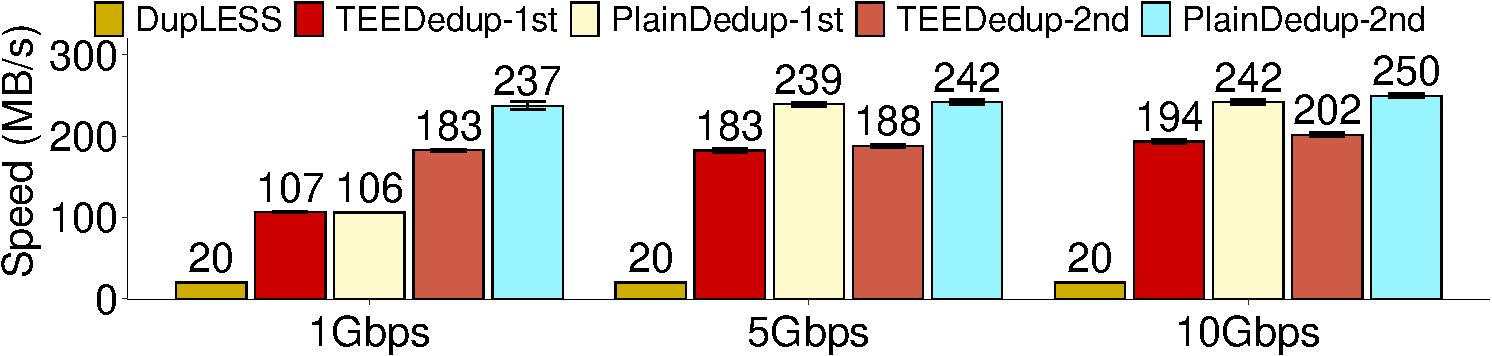
\includegraphics[width=0.646\textwidth]{pic/sgxdedup/plot/exp_b1/upload_network_speed_bar.pdf}
    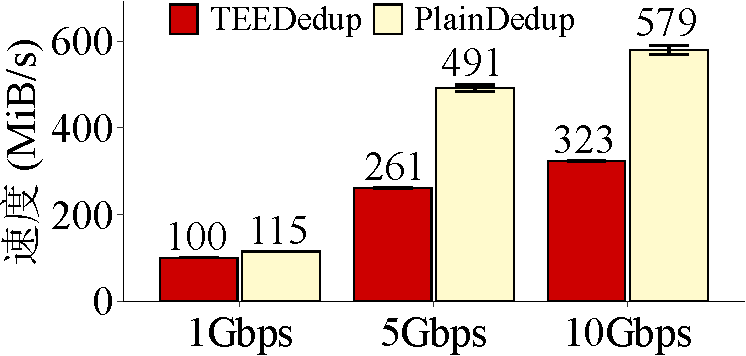
\includegraphics[width=0.324\textwidth]{pic/sgxdedup/plot/exp_b1/download_network_speed_bar.pdf}
    \\
    \hspace{1.1in} {\small (a) 上传} \hspace{1.9in}
    {\small (b) 下载}\\
    \caption{(Exp\#7)单客户端在不同网络速度下的上传/下载性能(由于DupLESS两轮上传速度相当,且其下载速度与\sysnameS 相当,此处并未展示相关结果以便更清晰展示对比结果)}
    \label{fig:sgxdedup-singleClientThroughput}
\end{figure}

图~\ref{fig:sgxdedup-singleClientThroughput}(a)显示了通过\textit{trickle}\cite{eriksen05}控制的不同网络带宽下的上传速度。在第一轮上传中,当网络带宽为1\,Gbps时,\sysnameS (106.6\,MiB/s)和PlainDedup(106.2\,MiB/s)的上传速度均受网络带宽制约,而DupLESS(20.1\,MiB/s)的性能瓶颈在于基于OPRF-RSA的密钥生成(参见Exp\#1)。当网络带宽增加到10\,Gbps(本地局域网测试平台的默认带宽)时,\sysnameS 和PlainDedup的上传速度分别达到193.6\,MiB/s和242.0\,MiB/s,而DupLESS的上传速度稳定在20.0\,MiB/s。对于第二轮上传,由于DupLESS性能瓶颈为数据块密钥生成,其上传速度与第一轮相同。而\sysnameS 和PlainDedup由于不再需要上传任何数据块,其上传速度受网络带宽的影响较小。平均而言,\sysnameS 在第一轮和第二轮上传中分别比DupLESS实现了8.1倍和9.6倍的性能提升。即使与不安全的PlainDedup相比,\sysnameS 也只会导致两轮上传速度分别下降约17.5\%和21.4\%。这些开销来自于\sysnameS 中的安全机制(包括密钥生成、数据块加密和所有权证明)。

图~\ref{fig:sgxdedup-singleClientThroughput}(b)显示了不同网络带宽下的下载速度。随着网络带宽增加到10\,Gbps,\sysnameS 和DupLESS的下载性能均达到323.1\,MiB/s。相较于PlainDedup下降了约44.2\%,其原因是作为加密后重复数据删除系统,它们首先下载并解密文件元数据然后再下载密文数据块(PlainDedup的可由云服务端直接读取文件元数据进行文件下载)。

\paragraph*{Exp\#8(云环境上传/下载性能)。}本文扩展Exp\#7,评估在真实云环境部署中的\sysnameS 的上传/下载速度。具体来说,本文将客户端和密钥服务器部署在本地局域网测试平台(\S\ref{sec:sgxdedup-evaluation})中,并通过互联网将客户端连接到部署在阿里云商的云服务端。本文使用阿里云\textit{ecs.c6e.xlarge}云服务器部署云服务端,其配备四核3.2GHz虚拟CPU(其底层物理平台为Intel Xeon Cascade Lake Platinum 8269CY),以及8GB内存。本文以阿里云通用文件存储(\textit{Alibaba General Purpose NAS})作为存储后端。该存储后端拥有20000\,IOPS的4\,K随机读写性能。

本文直接读取磁盘上的随机文件进行上传操作(与Exp\#7不同,后者在上传之前将文件加载到客户端的内存中),并在云服务端将收到的数据文件存储于通用文件存储中。本文使用最轻量化的\textit{scp}网络传输工具将测试的2\,GiB随机文件上传到云服务端作为互联网环境下的网络传输速率基准。

\begin{table}[!htb]
    \small
    \centering
    \renewcommand{\arraystretch}{1.05}
    \begin{tabular}{cccc}
        \toprule
        {\bf 方案}          & {\bf 第一轮上传(非重复数据)}        & {\bf 第二轮上传(重复数据)} & {\bf 下载}     \\
        \midrule
        网络带宽            & \multicolumn{3}{c}{11.9 $\pm$ 0.03}                                               \\  
        \sysnameS           & 11.4 $\pm$ 0.3                      & 104.3 $\pm$ 1.2            & 10.1 $\pm$ 0.1 \\ 
        \textit{PlainDedup} & 11.6 $\pm$ 0.1                      & 120.1 $\pm$ 1.4            & 11.3 $\pm$ 0.3 \\
        DupLESS             & \multicolumn{2}{c}{10.8 $\pm$ 0.2}  & 10.1 $\pm$ 0.1                              \\
        \bottomrule
    \end{tabular}
    \caption{(Exp\#8)云环境部署下\sysnameS 的上传/下载性能(单位:MiB/s)}
    \label{tab:sgxdedup-real-cloud}
\end{table}

表~\ref{tab:sgxdedup-real-cloud}显示了测试结果。在第一轮上传中,所有系统的性能(\sysnameS 为11.4\,MiB/s,PlainDedup为11.6\,MiB/s,DupLESS为10.8\,MiB/s)均受限于互联网网络带宽(11.9\,MiB/s)。在第二轮上传中,\sysnameS 实现了104.3\,MiB/s的上传速度,与DupLESS相比提升了9.7倍,与PlainDedup相比下降了13.2\%。这里的性能差异比Exp\#7中得到的结果要小,是因为\sysnameS 和PlainDedup受客户端磁盘I/O性能的限制。在下载中,这三个系统的性能再次受到互联网网络带宽的限制。此外,由于\sysnameS 和DupLESS先下载并处理文件元数据后再下载数据块并解密(参见Exp\#7),它们的下载性能相较于PlainDedup降低了10.6\%。

\paragraph*{Exp\#9(多客户端上传/下载性能)。}本文对\sysnameS 对多个客户端并发上传/下载的扩展性及其性能进行测试分析。本实验专注于\sysnameS,并将密钥安全区配置为在第一轮上传后为每个客户端同等的使用推测性加密(离线生成等量的加解密掩码)。本文将网络带宽固定为10\,Gbps,并评估所有客户端完成上传/下载的总体速度(即,所有客户端总操作数据量与从所有客户端开始上传/下载到最后一个客户端完成操作的时间的比值)。

图~\ref{fig:sgxdedup-multiClientThroughput}显示了多达10个客户端的测试结果。在第一轮上传中,由于客户端对云服务端的资源竞争,总体上传速度在7个客户端时达到峰值(637.0\,MiB/s),随后下降到10个客户端时的620.3\,MiB/s。同样,由于多个客户端的读取竞争,总下载速度最终下降到408.8\,MiB/s。而在第二轮上传中,由于不再需要向云服务端写入任何数据块,总体速度随着客户端数量增加而增加,最终在10个客户端时达到峰值1277.1\,MiB/s。

\paragraph*{Exp\#10(微基准性能测试)。}本文将\sysnameS 中各个步骤的计算时间开销分解以探究不同步骤的性能。假设密钥服务器及密钥安全区已启动并完成初始化,本文关注单个客户端的初始化(Initialization)和上传过程中各个步骤的时间开销。初始化过程客户端装载并启动所有权证明安全区。上传过程包括以下步骤:(1)数据分块(\textit{Chunking}),将输入文件划分为可变的小的明文数据块;(2)明文数据块指纹计算(\textit{Fingerprinting-p}),计算明文数据块的指纹,用于消息锁加密密钥生成;(3)密钥生成(\textit{Key generation}),客户端与密钥安全区生成消息锁加密密钥;(4)数据块加密(\textit{Encryption}),使用步骤3生成的消息锁加密密钥加密明文数据块;(5)密文数据块指纹计算(\textit{Fingerprinting-c}),所有权证明安全区计算密文数据块的指纹; (6)密文数据块指纹签名(\textit{Signing}),所有权证明安全区计算密文数据块指纹的签名;(7)云服务端验证(\textit{Verification}),云服务端基于签名验证接收到的指纹的真实性;(8)重复数据删除查询(\textit{Deduplication}),云服务端检测重复的密文数据块并通知客户端;(9)数据传输(\textit{Transfer}),上传非重复的密文数据块及文件元数据。

\begin{table}[!htb]
    \small
    \centering
    % \setlength{\tabcolsep}{5pt}
    % \renewcommand{\arraystretch}{1.05}
    \begin{tabular}{|c|c|c|c|}
        \hline
        \multicolumn{2}{|@{\,}c|}{\textbf{步骤/操作}} & \multicolumn{1}{l|}{\hspace{.5em}\textbf{第一轮上传(非重复数据)}} & 
        \multicolumn{1}{c|}{\textbf{第二轮上传(重复数据)}}                                                                                                                \\ \hline \hline
        \multicolumn{2}{|@{\,}c|}{初始化}             & 9.38 $\pm$
        2.72\,s                                       & 0.80 $\pm$ 0.004\,s                                                                                               \\ \hline
        \hline
        \multicolumn{2}{|c|}{数据分块}                & 
        \multicolumn{2}{c|}{3.77 $\pm$ 0.15\,ms }                                                                                                                         \\ \hline 
        \multicolumn{2}{|c|}{明文块指纹计算}
                                                      & 
        \multicolumn{2}{c|}{3.24 $\pm$ 0.28\,ms}                                                                                                                          \\ \hline
        \multicolumn{2}{|c|}{密钥生成}                & 
        0.31 $\pm$ 0.01\,ms                           & 0.18
        $\pm$ 0.01\,ms                                                                                                                                                    \\ \hline
        \multicolumn{2}{|c|}{数据块加密}              & 
        \multicolumn{2}{c|}{2.47 $\pm$ 0.10\,ms }                                                                                                                         \\ \hline
        \multirow{3}{*}{所有权证明}                   & 密文块指纹计算                                                    & \multicolumn{2}{c|}{3.28 $\pm$ 0.01\,ms }     \\ \cline{2-4}
                                                      & 指纹签名                                                          & \multicolumn{2}{c|}{0.01 $\pm$ 0.00004\,ms }  \\ \cline{2-4}
                                                      & 云服务端验证                                                      & \multicolumn{2}{c|}{0.005 $\pm$ 0.00003\,ms } \\ \hline
        \multicolumn{2}{|c|}{重复数据删除}            & \multicolumn{1}{c|}{0.38 $\pm$ 0.03\,ms }                         & 0.48 $\pm$ 0.03\,ms                           \\ \hline
        \multicolumn{2}{|c|}{数据传输}                & \multicolumn{1}{c|}{1.29 $\pm$ 0.09\,ms }                         & 0.05 $\pm$ 0.01\,ms                           \\ \hline
    \end{tabular}
    \caption{(Exp\#10)每处理1\,MiB数据时各步骤的时间开销}
    \label{tab:sgxdedup-system-breakdown}
\end{table}

表~\ref{tab:sgxdedup-system-breakdown}显示了每处理结1\,MiB文件数据时各个步骤的时间开销结果。初始化过程在第一轮上传时非常耗时,这是因为它需要联系Intel认证服务以检查所有权证明安全区的完整性。当客户端再次重启时,由于不再需要执行远程认证(\S\ref{subsec:sgxdedup-enclave-management}),初始化时间减少91.5\%。

实验发现基于TEE的服务器辅助密钥生成步骤是高效的,且最多占用整个上传时间的2.1\%。通过推测性加密,\sysnameS 进一步将密钥生成时间减少了41.9\%(第二轮相较于第一轮)。此外,数据所有权证明步骤占用了总上传时间的24.4\%,而所有权证明中的主要计算开销是密文数据块的指纹计算,该步骤对于之后的基于密文数据块的重复数据删除查询时必要的。通过轻量级的签名和验证步骤(最多占用总上传时间的0.1\%),本文可以保护源端重复数据删除免受伪造所有权的侧信道攻击,同时将重复数据的上传时间开销降低96.1\%。

